\documentclass[11pt, aspectratio=169]{beamer}
\usepackage[T1]{fontenc}
\usepackage[scaled]{helvet} 
\renewcommand\familydefault{\sfdefault}
\usepackage{graphicx}
\usepackage{booktabs}
\usepackage{tabularx}
\usepackage{amssymb} 
\usepackage{tikz}
\usetikzlibrary{arrows.meta, positioning, calc, decorations.pathreplacing, shadows, shapes.geometric}

% ---------- Academic, Traditional Palette ----------
% A classic academic scheme using Deep Navy, Maroon, and Slate.
\definecolor{primary}{RGB}{17, 34, 85}      % Deep Navy Blue (Formal, institutional)
\definecolor{accentA}{RGB}{138, 21, 56}     % Maroon / Burgundy (Classic academic accent)
\definecolor{accentB}{RGB}{85, 107, 130}    % Slate Grey/Blue (Secondary structure)
\definecolor{accentC}{RGB}{176, 188, 199}   % Light Slate (Soft accents)
\definecolor{bglight}{RGB}{250, 249, 246}   % Alabaster / Cream (Softer reading bg)

% ---------- Modern Flat Theme Settings ----------
\setbeamertemplate{navigation symbols}{}
\setbeamercolor{background canvas}{bg=bglight}

% Typography & Colors
\setbeamercolor{normal text}{fg=black!85}
\setbeamercolor{structure}{fg=primary}
\setbeamercolor{alerted text}{fg=accentA}
\setbeamerfont{title}{size=\Huge, series=\bfseries}
\setbeamerfont{frametitle}{size=\Large, series=\bfseries}
\setbeamercolor{title}{fg=primary}
\setbeamercolor{section in toc}{fg=primary}
\setbeamercolor{subsection in toc}{fg=black!60}
\setbeamertemplate{section in toc}[sections numbered]
\setbeamertemplate{subsection in toc}[subsections numbered]

% Itemize style
\setbeamertemplate{itemize item}{\color{accentA}$\blacktriangleright$}
\setbeamertemplate{itemize subitem}{\color{accentB}$\bullet$}

% Custom Frame Title
\setbeamertemplate{frametitle}{
    \nointerlineskip
    \begin{beamercolorbox}[wd=\paperwidth,ht=3.5ex,dp=1.2ex]{frametitle}
        \hspace*{2ex}\textcolor{primary}{\textbf{\insertframetitle}}
    \end{beamercolorbox}
    \vspace*{-1pt}
    \begin{beamercolorbox}[wd=\paperwidth,ht=0.25ex]{frametitle accent}
    \end{beamercolorbox}
}
\setbeamercolor{frametitle}{bg=white}
\setbeamercolor{frametitle accent}{bg=accentA}

% Custom Footline
\setbeamertemplate{footline}{
    \begin{beamercolorbox}[wd=\paperwidth,ht=2.5ex,dp=1.2ex]{footline}
        \hspace*{3ex}\textbf{\insertshortauthor} \hfill \insertshorttitle \hfill \textbf{\insertframenumber~|~\inserttotalframenumber}\hspace*{3ex}
    \end{beamercolorbox}
}
\setbeamercolor{footline}{bg=primary, fg=white}

% Blocks
\setbeamertemplate{blocks}[rounded][shadow=true]
\setbeamercolor{block title}{bg=primary, fg=white}
\setbeamercolor{block body}{bg=white, fg=black!85}

% ---------- Presentation Metadata ----------
\title[Pancasila \& UUD 1945]{Penerapan Nilai Pancasila\\\& Dinamika UUD NRI Tahun 1945}
\author[Kelompok 2]{Aliif $\cdot$ Avis $\cdot$ Azzahra $\cdot$ Regita $\cdot$ Wisam}
\institute[SMK]{SMK Plus Pratama Adi}
\date{\today}

\begin{document}

% =========================================================
% SLIDE 1 -- TITLE
\begin{frame}[plain]
    \begin{tikzpicture}[remember picture, overlay]
        \fill[primary] (current page.south west) rectangle ([xshift=1.5cm]current page.north west);
        \fill[accentA] ([xshift=1.5cm]current page.south west) rectangle ([xshift=1.8cm]current page.north west);
        \fill[accentB] ([xshift=1.8cm]current page.south west) rectangle ([xshift=2.0cm]current page.north west);
    \end{tikzpicture}
    \vspace*{0.5cm}
    \begin{flushleft}
        \hspace*{2.5cm}
        \begin{minipage}{0.8\textwidth}
            {\usebeamerfont{title}\usebeamercolor[fg]{title}\inserttitle\par}
            \vspace{0.6cm}
            {\large\textbf{\insertauthor}\par}
            \vspace{0.2cm}
            {\small\textcolor{black!60}{\insertinstitute} ~|~ \insertdate\par}
        \end{minipage}
    \end{flushleft}
\end{frame}

% =========================================================
% SLIDE 2 -- TOC
\begin{frame}{Contents}
    \begin{columns}
        \begin{column}{0.8\textwidth}
            \tableofcontents
        \end{column}
    \end{columns}
\end{frame}

% =========================================================
\section{Penerapan Nilai-Nilai Pancasila}

% SLIDE 4 -- 4 Kausa
\begin{frame}{Asal Mula Langsung}
    \small Menurut Kaelan (2020) mengutip Notonagoro, asal mula langsung Pancasila dibedakan menjadi:

    \vspace{4mm}
    \begin{center}
    \resizebox{0.98\linewidth}{!}{%
    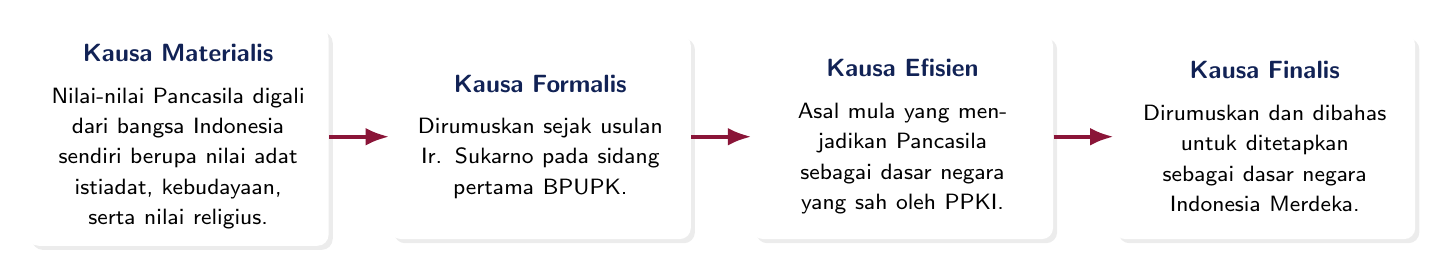
\begin{tikzpicture}[font=\small,
        kausabox/.style={rectangle, rounded corners=4pt, draw=none, fill=white,
                     drop shadow={opacity=0.15, shadow xshift=1.5pt, shadow yshift=-1.5pt},
                     text width=3.4cm, minimum height=2.6cm, align=center, inner sep=6pt}
    ]
        \node[kausabox] (m) at (0,0)    {\textcolor{primary}{\textbf{Kausa Materialis}}\\[4pt]\footnotesize Nilai-nilai Pancasila digali dari bangsa Indonesia sendiri berupa nilai adat istiadat, kebudayaan, serta nilai religius.};
        \node[kausabox] (f) at (4.6,0) {\textcolor{primary}{\textbf{Kausa Formalis}}\\[4pt]\footnotesize Dirumuskan sejak usulan Ir. Sukarno pada sidang pertama BPUPK.};
        \node[kausabox] (e) at (9.2,0) {\textcolor{primary}{\textbf{Kausa Efisien}}\\[4pt]\footnotesize Asal mula yang menjadikan Pancasila sebagai dasar negara yang sah oleh PPKI.};
        \node[kausabox] (t) at (13.8,0) {\textcolor{primary}{\textbf{Kausa Finalis}}\\[4pt]\footnotesize Dirumuskan dan dibahas untuk ditetapkan sebagai dasar negara Indonesia Merdeka.};
        \foreach \a/\b in {m/f, f/e, e/t}
            \draw[-{Latex[length=3mm]}, line width=1.5pt, accentA] (\a) -- (\b);
    \end{tikzpicture}}
    \end{center}
\end{frame}

% SLIDE 5 -- 3 tingkatan nilai
\begin{frame}{Tataran Nilai Ideologi Pancasila}
    \begin{columns}[c] 
        \begin{column}{0.55\textwidth}
            \small
            Nilai-nilai ideologi Pancasila dibedakan menjadi tiga tataran:

            \vspace{3mm}
            \textbf{\color{primary}Nilai Dasar}: Nilai fundamental dan universal (Ketuhanan, Kemanusiaan, Persatuan, Kerakyatan, Keadilan).
            
            \vspace{2mm}
            \textbf{\color{accentB}Nilai Instrumental}: Penjabaran nilai dasar dalam bentuk peraturan perundang-undangan dan kebijakan.
            
            \vspace{2mm}
            \textbf{\color{accentA}Nilai Praksis}: Realisasi nilai-nilai dalam kehidupan bermasyarakat, berbangsa, dan bernegara.
        \end{column}
        \begin{column}{0.42\textwidth}
            \centering
            \resizebox{0.9\linewidth}{!}{%
            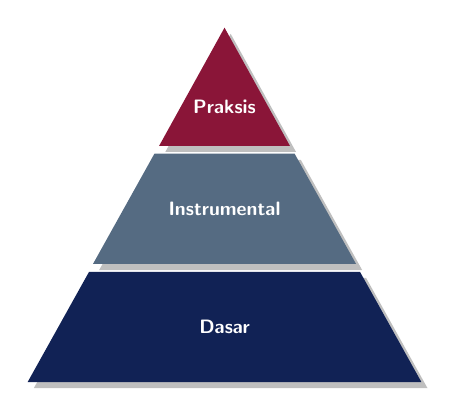
\begin{tikzpicture}[font=\footnotesize]
                % Bottom Layer (Nilai Dasar)
                \fill[primary, drop shadow] (-2.5,0) -- (2.5,0) -- (1.72,1.4) -- (-1.72,1.4) -- cycle;
                % Middle Layer (Instrumental)
                \fill[accentB, drop shadow] (-1.67,1.5) -- (1.67,1.5) -- (0.89,2.9) -- (-0.89,2.9) -- cycle;
                % Top Layer (Praksis)
                \fill[accentA, drop shadow] (-0.83,3.0) -- (0.83,3.0) -- (0,4.5) -- cycle;
                
                \node[font=\bfseries\scriptsize, text=white] at (0,0.7) {Dasar};
                \node[font=\bfseries\scriptsize, text=white] at (0,2.2) {Instrumental};
                \node[font=\bfseries\scriptsize, text=white] at (0,3.5) {Praksis};
            \end{tikzpicture}}
        \end{column}
    \end{columns}
\end{frame}

% =========================================================
\subsection{Pembudayaan Pancasila}

% SLIDE 7 -- pembudayaan & 5 jalur
\begin{frame}{Pembudayaan Pancasila}
    \small Menurut Yudi Latif (2020), pembudayaan Pancasila ditempuh melalui tiga ranah peradaban: \textbf{Ranah Keyakinan}, \textbf{Ranah Pengetahuan}, dan \textbf{Ranah Tindakan}. Terdapat jalur utama peradaban Pancasila:

    \vspace{4mm}
    \begin{center}
    \resizebox{0.95\linewidth}{!}{%
    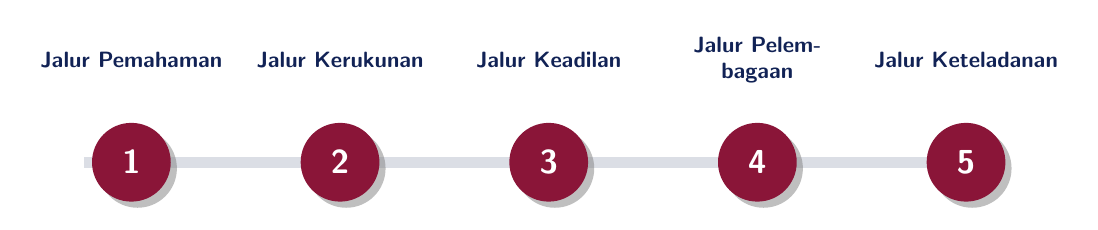
\begin{tikzpicture}[font=\small]
        \draw[line width=4pt, primary!15] (-0.6,0) -- (10.6,0);
        \foreach \x/\num/\lbl in {
            0/{1}/{Jalur Pemahaman},
            2.65/{2}/{Jalur Kerukunan},
            5.3/{3}/{Jalur Keadilan},
            7.95/{4}/{Jalur Pelembagaan},
            10.6/{5}/{Jalur Keteladanan}}
        {
            \node[circle, fill=accentA, text=white, font=\bfseries\large, minimum size=1cm, drop shadow] at (\x,0) {\num};
            \node[font=\bfseries\footnotesize, align=center, text width=2.4cm, text=primary] at (\x,1.3) {\lbl};
        }
    \end{tikzpicture}}
    \end{center}
    \vspace{3mm}
    \footnotesize\textit{\color{black!60}Catatan Kelembagaan: Pemerintah membentuk Badan Pembinaan Ideologi Pancasila (BPIP) pada 28 Februari 2018 berdasarkan Peraturan Presiden Nomor 7 Tahun 2018.}
\end{frame}

% =========================================================
\subsection{Contoh Penerapan Nilai-Nilai Pancasila}

% SLIDE 8 -- pengamalan sehari-hari
\begin{frame}{Contoh Penerapan Nilai-Nilai Pancasila}
    \begin{columns}[c]
        \begin{column}{0.4\textwidth}
            \centering
            \resizebox{0.9\linewidth}{!}{%
            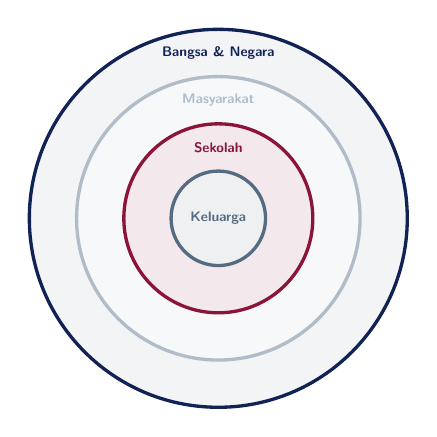
\begin{tikzpicture}[font=\scriptsize]
                % Concentric circles centered at 0,0
                \filldraw[fill=primary!5, draw=primary, line width=1.2pt] (0, 0) circle (2.4);
                \filldraw[fill=accentC!10, draw=accentC, line width=1.2pt] (0, 0) circle (1.8);
                \filldraw[fill=accentA!10, draw=accentA, line width=1.2pt] (0, 0) circle (1.2);
                \filldraw[fill=accentB!10, draw=accentB, line width=1.2pt] (0, 0) circle (0.6);
                
                \node[font=\bfseries\tiny, text=accentB] at (0, 0) {Keluarga};
                \node[font=\bfseries\tiny, text=accentA] at (0, 0.9) {Sekolah};
                \node[font=\bfseries\tiny, text=accentC] at (0, 1.5) {Masyarakat};
                \node[font=\bfseries\tiny, text=primary] at (0, 2.1) {Bangsa \& Negara};
            \end{tikzpicture}}
        \end{column}
        \begin{column}{0.6\textwidth}
            \scriptsize 
            \textbf{\color{accentB}Di Lingkungan Keluarga:}
            \begin{itemize}
                \setlength{\itemsep}{1pt}
                \setlength{\parskip}{0pt}
                \item Memecahkan masalah dengan berdiskusi bersama anggota keluarga.
                \item Membantu menyelesaikan pekerjaan di rumah.
            \end{itemize}

            \vspace{1.5mm}
            \textbf{\color{accentA}Di Lingkungan Sekolah:}
            \begin{itemize}
                \setlength{\itemsep}{1pt}
                \setlength{\parskip}{0pt}
                \item Disiplin mematuhi tata tertib sekolah.
                \item Melaporkan terjadinya kasus perundungan kepada guru.
            \end{itemize}

            \vspace{1.5mm}
            \textbf{\color{accentC}Di Lingkungan Masyarakat:}
            \begin{itemize}
                \setlength{\itemsep}{1pt}
                \setlength{\parskip}{0pt}
                \item Mengutamakan musyawarah dalam pengambilan keputusan bersama.
                \item Rukun dengan sesama tetangga.
            \end{itemize}

            \vspace{1.5mm}
            \textbf{\color{primary}Di Lingkungan Bangsa dan Negara:}
            \begin{itemize}
                \setlength{\itemsep}{1pt}
                \setlength{\parskip}{0pt}
                \item Menyampaikan pendapat atau aspirasi secara bertanggung jawab.
                \item Mematuhi hukum yang berlaku.
            \end{itemize}
        \end{column}
    \end{columns}
\end{frame}

% =========================================================
\section{Dinamika Pelaksanaan UUD NRI Tahun 1945}
\subsection{Pentingnya Konstitusi}

% SLIDE 9 -- apa itu konstitusi
\begin{frame}{Pentingnya Konstitusi}
    \small Istilah konstitusi berasal dari bahasa Prancis (constituer) dan Inggris (constitution) yang berarti membentuk. Konstitusi merupakan peraturan atau hukum dasar tertinggi yang dijadikan pegangan dalam penyelenggaraan pemerintahan negara.

    \vspace{4mm}
    \begin{columns}[T]
        \begin{column}{0.48\textwidth}
            \begin{block}{\centering\textbf{Konstitusi Tertulis}}
                \footnotesize Documentary constitution, contohnya UUD NRI Tahun 1945.
            \end{block}
        \end{column}
        \begin{column}{0.48\textwidth}
            \begin{block}{\centering\textbf{Konstitusi Tidak Tertulis}}
                \footnotesize Non-documentary constitution atau konvensi (kebiasaan ketatanegaraan).
            \end{block}
        \end{column}
    \end{columns}
    \vspace{4mm}
    \footnotesize Contoh kebiasaan ketatanegaraan (konvensi) di Indonesia adalah Pidato Presiden setiap tanggal 16 Agustus di depan sidang paripurna DPR.
\end{frame}

% =========================================================
\subsection{Sejarah Penyusunan UUD NRI Tahun 1945}

% SLIDE 10 -- timeline BPUPK-PPKI
\begin{frame}{Sejarah Penyusunan UUD NRI Tahun 1945}
    \small UUD NRI Tahun 1945 dirancang sejak tanggal 29 Mei 1945 sampai 16 Juli 1945 oleh BPUPK.

    \vspace{2mm}
    \begin{center}
    \resizebox{\linewidth}{!}{%
    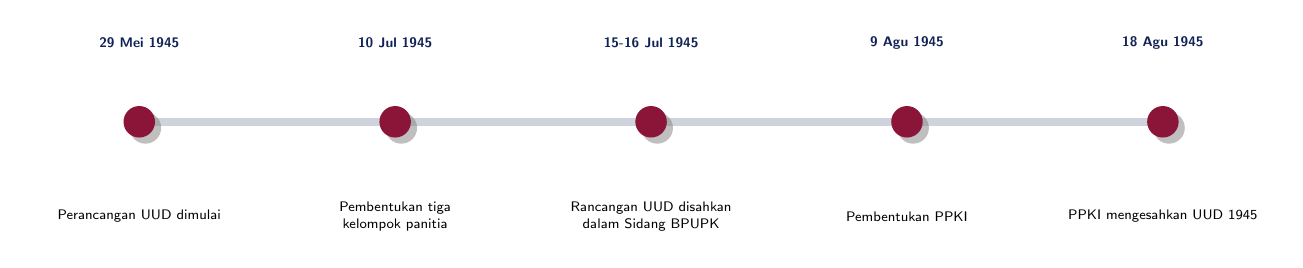
\begin{tikzpicture}[font=\footnotesize]
        \draw[line width=3pt, primary!20] (0,0) -- (13,0);
        \foreach \x/\date/\desc in {
            0/{29 Mei 1945}/{Perancangan UUD dimulai},
            3.25/{10 Jul 1945}/{Pembentukan tiga kelompok panitia},
            6.5/{15-16 Jul 1945}/{Rancangan UUD disahkan dalam Sidang BPUPK},
            9.75/{9 Agu 1945}/{Pembentukan PPKI},
            13/{18 Agu 1945}/{PPKI mengesahkan UUD 1945}}
        {
            \node[circle, fill=accentA, minimum size=0.4cm, drop shadow] at (\x,0) {};
            \node[font=\bfseries\tiny, align=center, text width=2.5cm, text=primary] at (\x,1.0) {\date};
            \node[font=\tiny, align=center, text width=2.6cm] at (\x,-1.2) {\desc};
        }
    \end{tikzpicture}}
    \end{center}
    \vspace{2mm}
    \footnotesize Pada tanggal 10 Juli 1945 dibentuk tiga kelompok panitia:
    \textbf{Panitia Perancang Hukum Dasar} (diketuai Ir. Sukarno), \textbf{Panitia Perancang Keuangan dan Ekonomi} (diketuai Drs. Mohammad Hatta), dan \textbf{Panitia Perancang Pembelaan Tanah Air} (diketuai Abikoesno Tjokrosoejoso).
\end{frame}

% =========================================================
\subsection{Pembukaan UUD NRI Tahun 1945}

% SLIDE 12 -- 4 alinea
\begin{frame}{Isi dan Tujuan Pembukaan UUD NRI Tahun 1945}
    \small Menurut Kaelan (2020), makna per alinea Pembukaan UUD NRI 1945 adalah:
    
    \vspace{4mm}
    \begin{center}
    \resizebox{0.95\linewidth}{!}{%
    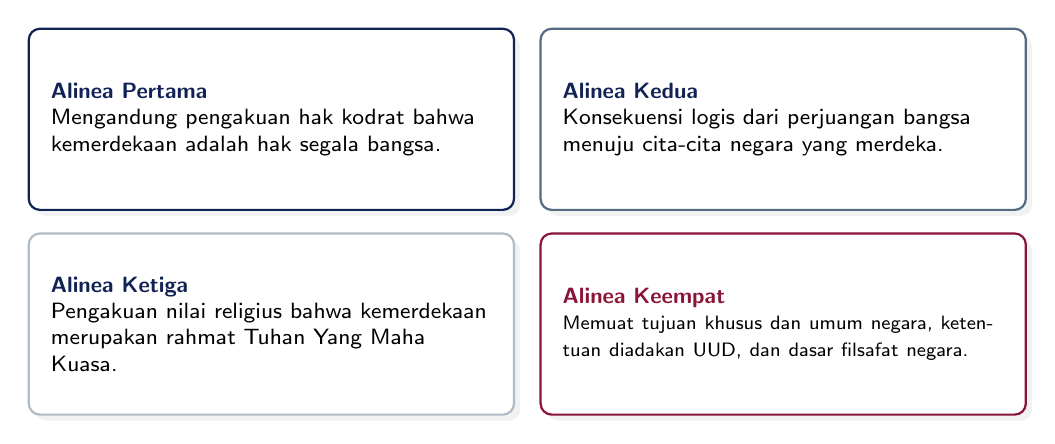
\begin{tikzpicture}[font=\footnotesize,
        box/.style={rectangle, rounded corners=4pt, draw=none, fill=white,
                    drop shadow={opacity=0.1}, text width=5.6cm, minimum height=2.3cm, align=left, inner sep=8pt}
    ]
        \node[box, draw=primary, thick] at (0,1.75)   {\textcolor{primary}{\textbf{Alinea Pertama}}\\ Mengandung pengakuan hak kodrat bahwa kemerdekaan adalah hak segala bangsa.};
        \node[box, draw=accentB, thick] at (6.5,1.75) {\textcolor{primary}{\textbf{Alinea Kedua}}\\ Konsekuensi logis dari perjuangan bangsa menuju cita-cita negara yang merdeka.};
        \node[box, draw=accentC, thick] at (0,-0.85)  {\textcolor{primary}{\textbf{Alinea Ketiga}}\\ Pengakuan nilai religius bahwa kemerdekaan merupakan rahmat Tuhan Yang Maha Kuasa.};
        \node[box, draw=accentA, thick] at (6.5,-0.85){\textcolor{accentA}{\textbf{Alinea Keempat}}\\ \scriptsize Memuat tujuan khusus dan umum negara, ketentuan diadakan UUD, dan dasar filsafat negara.};
    \end{tikzpicture}}
    \end{center}
\end{frame}

% SLIDE 13 -- kenapa ga bisa diubah + hubungan
\begin{frame}{Alasan Pembukaan UUD NRI 1945 Tidak Dapat Diubah}
    \footnotesize
    Secara formal-yuridis, kedudukannya bersifat tetap, kuat, dan terlekat erat pada keberadaan negara sebagai pokok kaidah negara yang fundamental (staatsfundamentalnorm). 
    
    Mengubah atau menghapus Pembukaan sama artinya dengan membubarkan Negara Kesatuan Republik Indonesia (NKRI).

    \vspace{4mm}
    \begin{center}
    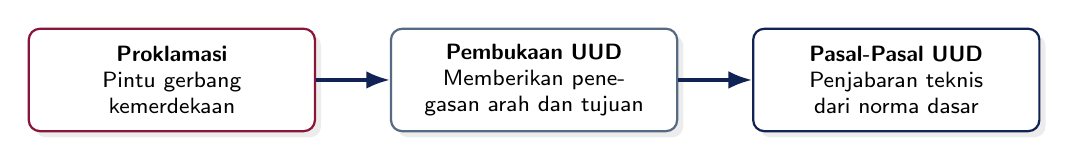
\begin{tikzpicture}[font=\footnotesize,
        b/.style={rectangle, rounded corners=4pt, draw=none, fill=white, drop shadow={opacity=0.15},
                  text width=3.4cm, minimum height=1.3cm, align=center}]
        \node[b, draw=accentA, thick] (p1) at (0,0) {\textbf{Proklamasi}\\\footnotesize Pintu gerbang kemerdekaan};
        \node[b, draw=accentB, thick] (p2) at (4.6,0) {\textbf{Pembukaan UUD}\\\footnotesize Memberikan penegasan arah dan tujuan};
        \node[b, draw=primary, thick] (p3) at (9.2,0) {\textbf{Pasal-Pasal UUD}\\\footnotesize Penjabaran teknis dari norma dasar};
        \draw[-{Latex[length=3mm]}, line width=1.2pt, primary] (p1) -- (p2);
        \draw[-{Latex[length=3mm]}, line width=1.2pt, primary] (p2) -- (p3);
    \end{tikzpicture}
    \end{center}
    \vspace{4mm}
    Empat Pokok Pikiran dalam Pembukaan UUD NRI Tahun 1945: \textbf{Persatuan}, \textbf{Keadilan Sosial}, \textbf{Kedaulatan Rakyat}, dan \textbf{Ketuhanan \& Kemanusiaan}.
\end{frame}

% =========================================================
\subsection{Dinamika Pelaksanaan UUD NRI Tahun 1945}

% SLIDE 14 -- 5 periode (timeline)
\begin{frame}{Dinamika Pelaksanaan UUD NRI Tahun 1945}
    \small Pelaksanaan UUD NRI Tahun 1945 telah mengalami dinamika dan beberapa kali pergantian akibat perkembangan politik nasional:

    \vspace{4mm}
    \begin{center}
    \resizebox{\linewidth}{!}{%
    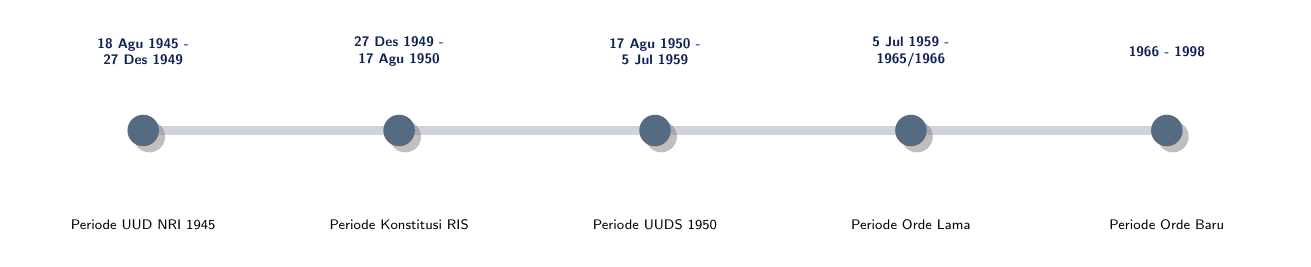
\begin{tikzpicture}[font=\footnotesize]
        \draw[line width=3pt, primary!20] (0,0) -- (13,0);
        \foreach \x/\th/\lbl in {
            0/{18 Agu 1945 -\\27 Des 1949}/{Periode UUD NRI 1945},
            3.25/{27 Des 1949 -\\17 Agu 1950}/{Periode Konstitusi RIS},
            6.5/{17 Agu 1950 -\\5 Jul 1959}/{Periode UUDS 1950},
            9.75/{5 Jul 1959 -\\1965/1966}/{Periode Orde Lama},
            13/{1966 - 1998}/{Periode Orde Baru}}
        {
            \node[circle, fill=accentB, minimum size=0.4cm, drop shadow] at (\x,0) {};
            \node[font=\bfseries\tiny, align=center, text width=2.6cm, text=primary] at (\x,1.0) {\th};
            \node[font=\tiny, align=center, text width=2.7cm] at (\x,-1.2) {\lbl};
        }
    \end{tikzpicture}}
    \end{center}
    \vspace{4mm}
    \footnotesize Dampak negatif Masa UUDS 1950: Sering terjadi pergantian kabinet (7 kali berganti dalam 9 tahun), menimbulkan ketidakharmonisan, dan kebuntuan Badan Konstituante.
\end{frame}

% =========================================================
\subsection{Pergantian dan Perubahan UUD NRI Tahun 1945}

% SLIDE 15 -- amandemen
\begin{frame}{Perubahan UUD NRI 1945 Era Reformasi (1999-2002)}
    \footnotesize
    Amandemen dilakukan sebanyak 4 kali untuk membatasi kekuasaan executive heavy, memperkuat perlindungan HAM, serta menegaskan otonomi daerah.
    
    Perubahan UUD dilakukan dengan cara addendum (mempertahankan naskah asli dan melampirkan naskah perubahan di bagian akhir).

    \vspace{4mm}
    \begin{center}
    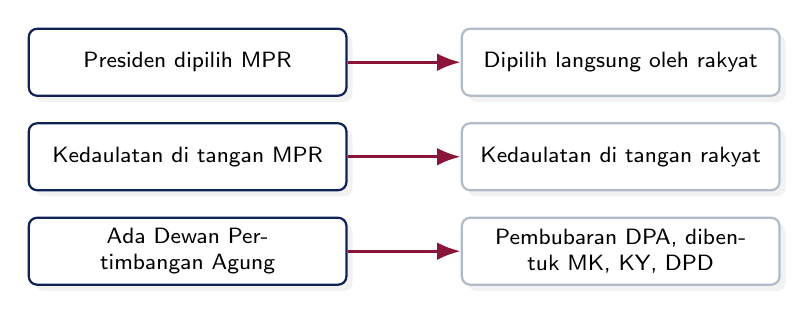
\begin{tikzpicture}[font=\footnotesize,
        n/.style={rectangle, rounded corners=3pt, draw=none, fill=white, drop shadow={opacity=0.1},
                  text width=3.8cm, minimum height=0.85cm, align=center}]
        \node[n, draw=primary, thick] (a1) at (0,1.6)   {Presiden dipilih MPR};
        \node[n, draw=accentC, thick] (a2) at (5.5,1.6) {Dipilih langsung oleh rakyat};
        \node[n, draw=primary, thick] (b1) at (0,0.4)   {Kedaulatan di tangan MPR};
        \node[n, draw=accentC, thick] (b2) at (5.5,0.4) {Kedaulatan di tangan rakyat};
        \node[n, draw=primary, thick] (c1) at (0,-0.8)  {Ada Dewan Pertimbangan Agung};
        \node[n, draw=accentC, thick] (c2) at (5.5,-0.8){Pembubaran DPA, dibentuk MK, KY, DPD};
        \foreach \a/\b in {a1/a2, b1/b2, c1/c2}
            \draw[-{Latex[length=3mm]}, line width=1.2pt, accentA] (\a) -- (\b);
    \end{tikzpicture}
    \end{center}
\end{frame}

% =========================================================
\subsection{Peran Mahkamah Konstitusi}

% SLIDE 16 -- MK
\begin{frame}{Peran Mahkamah Konstitusi}
    \vspace{2mm}
    \begin{center}
    \resizebox{0.75\linewidth}{!}{%
    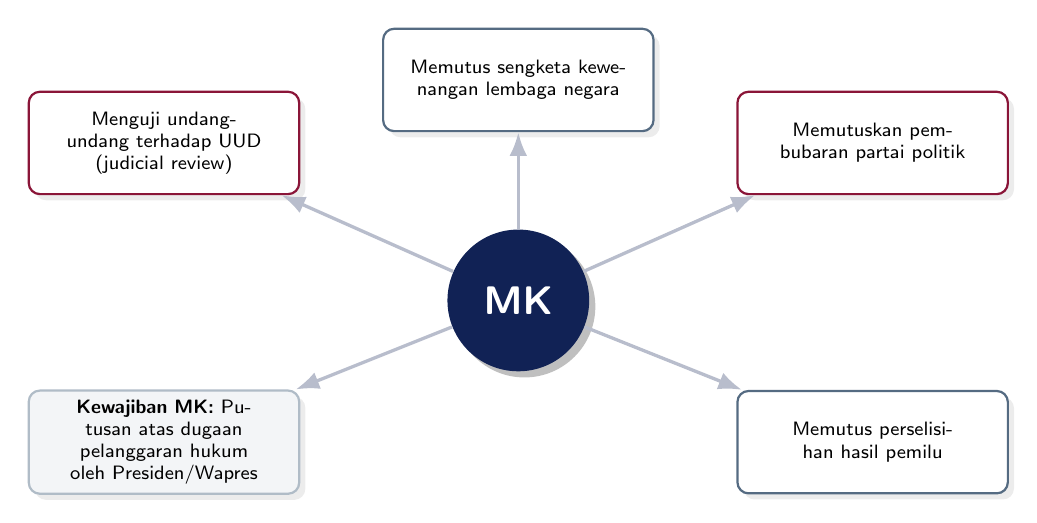
\begin{tikzpicture}[font=\footnotesize,
        center/.style={circle, draw=none, fill=primary, text=white, font=\bfseries\Large,
                       minimum size=1.8cm, drop shadow},
        leaf/.style={rectangle, rounded corners=4pt, draw=none, fill=white, drop shadow={opacity=0.15},
                     text width=3.2cm, minimum height=1.3cm, align=center, font=\scriptsize}
    ]
        \node[center] (mk) at (0,0) {MK};
        \node[leaf, draw=accentA, thick] (k1) at (-4.5,2.0) {Menguji undang-undang terhadap UUD\\(judicial review)};
        \node[leaf, draw=accentB, thick] (k2) at (0,2.8)    {Memutus sengketa kewenangan lembaga negara};
        \node[leaf, draw=accentA, thick] (k3) at (4.5,2.0)  {Memutuskan pembubaran partai politik};
        \node[leaf, draw=accentB, thick] (k4) at (4.5,-1.8) {Memutus perselisihan hasil pemilu};
        \node[leaf, draw=accentC, fill=accentC!15, thick] (kw) at (-4.5,-1.8)
            {\textbf{Kewajiban MK:} Putusan atas dugaan pelanggaran hukum oleh Presiden/Wapres};
            
        \foreach \n in {k1,k2,k3,k4,kw}
            \draw[-{Latex[length=3mm]}, line width=1.2pt, primary!30] (mk) -- (\n);
    \end{tikzpicture}}
    \end{center}
    \vspace{4mm}
    \footnotesize Pengadilan yang dilakukan oleh Mahkamah Konstitusi merupakan pengadilan tingkat pertama dan terakhir yang putusannya bersifat final.
\end{frame}

% =========================================================
\subsection{Hak dan Kewajiban Warga Negara}

% SLIDE 17 -- konsep hak & kewajiban
\begin{frame}{Hak dan Kewajiban Warga Negara}
    \begin{columns}[c]
        \begin{column}{0.55\textwidth}
            \small
            Hak berarti kepunyaan, kewenangan, kekuasaan untuk berbuat sesuatu, sedangkan kewajiban artinya sesuatu yang harus dilaksanakan.
            
            \vspace{3mm}
            Sifat pelaksanaan hak dan kewajiban:
            \begin{enumerate}
                \item Timbal balik dengan negara
                \item Kausalitas atau hubungan sebab akibat
                \item Tidak dapat dipisahkan
            \end{enumerate}

            \vspace{3mm}
            Hak dan kewajiban yang dijamin oleh UUD NRI Tahun 1945 disebut sebagai hak dan kewajiban konstitusional.
        \end{column}
        \begin{column}{0.45\textwidth}
            \centering
            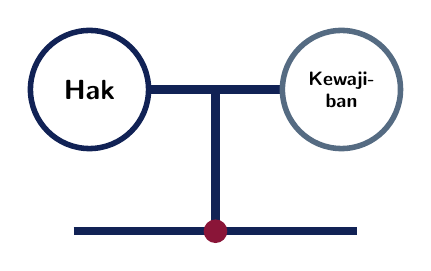
\begin{tikzpicture}[font=\small]
                \draw[line width=3pt, primary] (-1.8,0) -- (1.8,0);
                \draw[line width=3pt, primary] (0,0) -- (0,1.8);
                \draw[line width=3pt, primary] (0,1.8) -- (-1.6,1.8);
                \draw[line width=3pt, primary] (0,1.8) -- (1.6,1.8);
                
                \node[circle, draw=primary, line width=2pt, fill=white, minimum size=1.5cm, font=\bfseries] at (-1.6,1.8) {Hak};
                \node[circle, draw=accentB, line width=2pt, fill=white, minimum size=1.5cm, font=\bfseries\scriptsize, align=center] at (1.6,1.8) {Kewaji-\\ban};
                
                \fill[accentA] (0,0) circle[radius=0.15];
            \end{tikzpicture}
        \end{column}
    \end{columns}
\end{frame}

% SLIDE 18 -- pasal grid
\begin{frame}{Hak dan Kewajiban dalam UUD NRI Tahun 1945}
    \begin{center}
    \resizebox{0.95\linewidth}{!}{%
    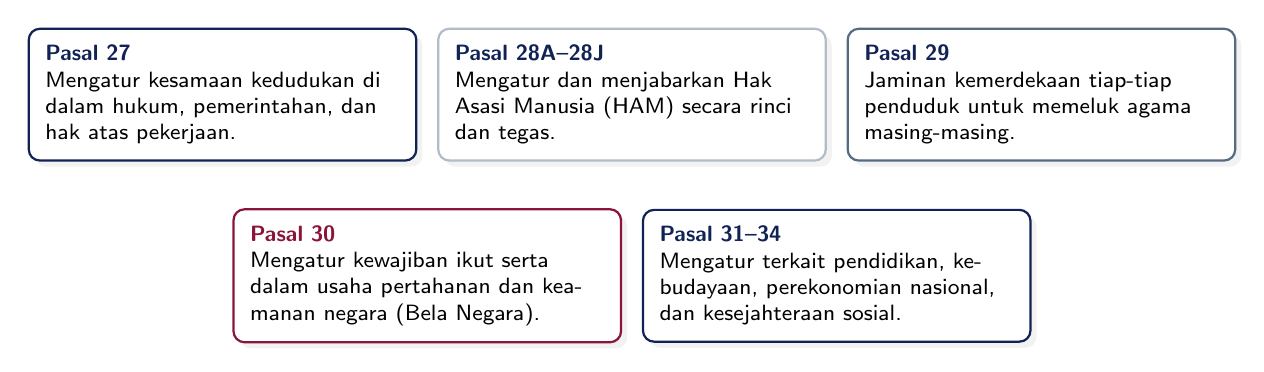
\begin{tikzpicture}[font=\footnotesize,
        p/.style={rectangle, rounded corners=4pt, draw=none, fill=white, drop shadow={opacity=0.1},
                  text width=4.5cm, minimum height=1.6cm, align=left, inner sep=6pt}]
        \node[p, draw=primary, thick] at (0,2.0)   {\textcolor{primary}{\textbf{Pasal 27}}\\\footnotesize Mengatur kesamaan kedudukan di dalam hukum, pemerintahan, dan hak atas pekerjaan.};
        \node[p, draw=accentC, thick] at (5.2,2.0) {\textcolor{primary}{\textbf{Pasal 28A--28J}}\\\footnotesize Mengatur dan menjabarkan Hak Asasi Manusia (HAM) secara rinci dan tegas.};
        \node[p, draw=accentB, thick] at (10.4,2.0){\textcolor{primary}{\textbf{Pasal 29}}\\\footnotesize Jaminan kemerdekaan tiap-tiap penduduk untuk memeluk agama masing-masing.};
        
        \node[p, draw=accentA, thick] at (2.6,-0.3)  {\textcolor{accentA}{\textbf{Pasal 30}}\\\footnotesize Mengatur kewajiban ikut serta dalam usaha pertahanan dan keamanan negara (Bela Negara).};
        \node[p, draw=primary, thick] at (7.8,-0.3){\textcolor{primary}{\textbf{Pasal 31--34}}\\\footnotesize Mengatur terkait pendidikan, kebudayaan, perekonomian nasional, dan kesejahteraan sosial.};
    \end{tikzpicture}}
    \end{center}
\end{frame}

% SLIDE 19 -- contoh sehari-hari
\begin{frame}{Contoh Hak dan Kewajiban Warga Negara Indonesia}
    \vspace{2mm}
    \begin{columns}[T]
        \begin{column}{0.48\textwidth}
            \begin{block}{\centering \textbf{Contoh Hak}}
                \footnotesize 
                \begin{itemize}
                    \item Memeluk dan menjalankan ibadah sesuai dengan agama dan kepercayaannya.
                    \item Menyuarakan pendapat secara lisan maupun tulisan.
                    \item Mendapatkan pendidikan dan pengajaran.
                    \item Memiliki kedudukan yang sama di dalam hukum dan mendapat perlindungan hukum.
                \end{itemize}
            \end{block}
        \end{column}
        \begin{column}{0.48\textwidth}
            \begin{block}{\centering \textbf{Contoh Kewajiban}}
                \footnotesize 
                \begin{itemize}
                    \item Membayar pajak dan retribusi yang ditetapkan pemerintah.
                    \item Taat dan patuh pada peraturan hukum yang berlaku.
                    \item Menghormati orang lain.
                    \item Ikut menjaga sarana dan fasilitas umum.
                \end{itemize}
            \end{block}
        \end{column}
    \end{columns}
\end{frame}

% =========================================================
% SLIDE 21 -- PENUTUP
\begin{frame}[plain]
    \begin{tikzpicture}[remember picture, overlay]
        \fill[primary] (current page.south west) rectangle (current page.north east);
    \end{tikzpicture}
    
    \begin{center}
        \vspace{1.5cm}
        \textcolor{white}{\Huge \textbf{Terima Kasih}}\\
        \vspace{0.8cm}
        
\begin{tikzpicture}
            \draw[thick, accentB!50] (0,0) -- (6,0);
        \end{tikzpicture}\\
        \begin{center}
            \textcolor{bglight}{Apakah Ada Pertanyaan?}
        \end{center}
        \vspace{0.5cm}
    \end{center}
\end{frame}

\end{document}
